\documentclass{article}
\usepackage[english]{babel}
\usepackage[a4paper, total={6in, 8in}]{geometry}
\usepackage{fancyhdr}
\setlength{\parskip}{0.5em}

% Mathematics packages
\usepackage{amsthm, amsmath, amssymb, amsfonts, nicefrac, mathpazo} 
\usepackage{graphicx}
\usepackage{subcaption}
\usepackage{csquotes}

% Coding colours
\usepackage{color}
\definecolor{codegreen}{rgb}{0,0.6,0}
\definecolor{codegray}{rgb}{0.5,0.5,0.5}
\definecolor{codepurple}{rgb}{0.58,0,0.82}
\definecolor{backcolour}{rgb}{0.95,0.95,0.92}
\definecolor{codeblue}{rgb}{0,0,1}
 
% Coding style
\usepackage{listings}
\lstdefinestyle{mystyle}{
    backgroundcolor=\color{backcolour},   
    commentstyle=\color{codegreen},
    keywordstyle=\color{codeblue},
    numberstyle=\tiny\color{codegray},
    stringstyle=\color{codepurple},
    basicstyle=\footnotesize,
    breakatwhitespace=false,         
    breaklines=true,                 
    captionpos=b,                    
    keepspaces=true,                 
    numbers=left,                    
    numbersep=5pt,                  
    showspaces=false,                
    showstringspaces=false,
    showtabs=false,                  
    tabsize=2
}
\lstset{style=mystyle}

% Easier to call Naturals, Integers and so on.
\newcommand{\N}{\mathbb{N}}
\newcommand{\Z}{\mathbb{Z}}
\newcommand{\Q}{\mathbb{Q}}
\newcommand{\C}{\mathbb{C}}
\newcommand{\ind}{1\hspace{-2.1mm}{1}} %Indicator Function
\newcommand{\I}{\mathtt{i}}
\newcommand{\EE}{\mathbb{E}}
\newcommand{\RR}{\mathbb{R}}
\newcommand{\PP}{\mathbb{P}}
\newcommand{\D}{\mathrm{d}}
\newcommand{\Xe}{X^{\varepsilon}}
\newcommand{\E}{\mathrm{e}}
\newcommand{\Tr}{\mathrm{Tr}}
\newcommand{\HH}{\mathrm{H}}
\newcommand{\sgn}{\mathrm{sgn}}
\newcommand{\atanh}{\mathrm{arctanh}}
\def\equalDistrib{\,{\buildrel \Delta \over =}\,}

% Writing Algorithms
\usepackage[]{algpseudocode}

%%%%%%%%%%%%%%%%%%%%%%%%%%%%%%%%%%%%%%%%%%%%%%%%%%%%%%%%%%%%
\title{M4N9: Project 0}
\author{Yadu Bhageria}
\date{February 2016}

%\pagestyle{fancy}
%\fancyhf{}
%\rhead{CID 00733164}
%\lhead{Yadu Bhageria}
\cfoot{\thepage}

%%%%%%%%%%%%%%%%%%%%%%%%%%%%%%%%%%%%%%%%%%%%%%%%%%%%%%%%%%%%
%%%%%%%%%%%%%%%%%%%%%%%%%%%%%%%%%%%%%%%%%%%%%%%%%%%%%%%%%%%%
\begin{document}
\lstset{language=Matlab}

\begin{titlepage}
    \begin{center}
    
        Coursework report presented for\\
        M4N9
        
        \vfill
        
        {\Huge Computational Linear Algebra\\ Project 2}
        
        
        \vspace{0.5cm}
        %subtitle?
        
        \vspace{1.5cm}
        
        {\Large Yadu \emph{Bhageria}}
        
        \vfill
        
        Mathematics Department\\
        Imperial College London\\
        United Kingdom\\
        \today
        
    \end{center}
\end{titlepage}
%%%%%%%%%%%%%%%%%%%%%%%%%%%%%%%%%%%%%%%%%%%%%%%%%%%%%%%%%%%%

\begin{enumerate}
%%%%%%%%%%%%%%%%%%%%%%%%%%%%%%%%%%%%%%%%%%%%%%%%%%%%%%%%%%%%
	\item \textbf{PageRank Algorithm}
	\begin{enumerate}
		%%%%%%%%%%%%%%%%%%%%%%%%%%%%%%%%%%%%%%%%%%%%%%%%%%%%%%%%%%%%	
		\item The algorithm page rank is using Power Iteration where the $k^\text{th}$ iteration is
		$$
			\textbf{x}^{(k+1)} = \textbf{P}^T \textbf{x}^{(k)}
		$$
		Also note since $\sum_{j=1}^N x_j = 1$ and the rows of $\textbf{P}^T$ sum to 1, $\textbf{x}^{(k+1)}$ is always normalized at each step of the algorithm.
		
		We know that power iteration is restricted to finding the eigenvector associated with the largest eigenvalue of the iterative matrix, $\textbf{P}^T$. In this case we, for the last iteration, l, in the algorithm
		 $$
		 	\textbf{P}^T \textbf{x}^{(l)} = \textbf{x}^{(l+1)}
		 $$
		 and 
		 $$
		 	|\textbf{x}^{(l+1)} - \textbf{x}^{(l)}| < \text{tolerance value}
		 $$
		 So $ \textbf{x}^{(l+1)} \approx \textbf{x}$ as well as $ \textbf{x}^{(l)} \approx \textbf{x}$. This means
		 $$
		 	\textbf{P}^T \textbf{x}^{(l)} \approx 1 \cdot \textbf{x}^{(l+1)} \implies \textbf{P}^T \textbf{x} \approx 1 \cdot \textbf{x}
		 $$
		 which is the eigenvalue equation for a matrix and vector. Thus the final state vector, $\textbf{x}$, is an eigenvector of $\textbf{P}^T$ with 1 as its corresponding eigenvalue, also the most dominant eigenvalue of $\textbf{P}^T$. \\
		 After having found $\textbf{x}$ the eigenvalue, $\lambda$, can be checked using the formula
		 $$
		 	\lambda = \textbf{x}	^T \textbf{P}^T \textbf{x}	 
		 $$
		 to see if it is equal to 1 and any variation that occurs in doing so.
		 \newpage
		%%%%%%%%%%%%%%%%%%%%%%%%%%%%%%%%%%%%%%%%%%%%%%%%%%%%%%%%%%%%
		\item List of the top 50 sites by their index is \\
			\begin{table}[h!]
			\centering
			\begin{tabular}{|c|c|c|c|} 
				\hline
				Position & Webpage Index & Position & Webpage Index \\
				\hline
				1 & 1489 & 26 & 10\\ 
				2 & 4392 & 27 & 103\\ 
				3 & 67 & 28 & 7\\ 
				4 & 6428 & 29 & 2218\\ 
				5 & 4824 & 30 & 1662\\ 
				6 & 2079 & 31 & 719\\ 
				7 & 1 & 32 & 148\\ 
				8 & 1490 & 33 & 7896\\ 
				9 & 1618 & 34 & 137\\ 
				10 & 2409 & 35 & 788\\ 
				11 & 18 & 36 & 6131\\ 
				12 & 1807 & 37 & 142\\ 
				13 & 998 & 38 & 4\\ 
				14 & 42 & 39 & 15\\ 
				15 & 212 & 40 & 8717\\ 
				16 & 1863 & 41 & 9\\ 
				17 & 1864 & 42 & 94\\ 
				18 & 1084 & 43 & 35\\ 
				19 & 1080 & 44 & 75\\ 
				20 & 127 & 45 & 2217\\ 
				21 & 8052 & 46 & 83\\ 
				22 & 7756 & 47 & 5754\\ 
				23 & 33 & 48 & 11\\ 
				24 & 1661 & 49 & 55\\ 
				25 & 2476 & 50 & 7801 \\
				\hline
			\end{tabular}
			\caption{Top 50 sites after running the PageRank algorithm for $\alpha = 0.85$, tolerance $= 10^{-8}$ and $\textbf{x}^{(0)} = \textbf{e}_1$}
			\end{table}
			
			The files \texttt{PageRank.m} and \texttt{q1b.m} produce these results. \texttt{tabletop50.m} is used to produce latex raw text for importing the top50 results into a \texttt{tex} file.
		%%%%%%%%%%%%%%%%%%%%%%%%%%%%%%%%%%%%%%%%%%%%%%%%%%%%%%%%%%%%
		\item  
			\begin{figure}[h]
				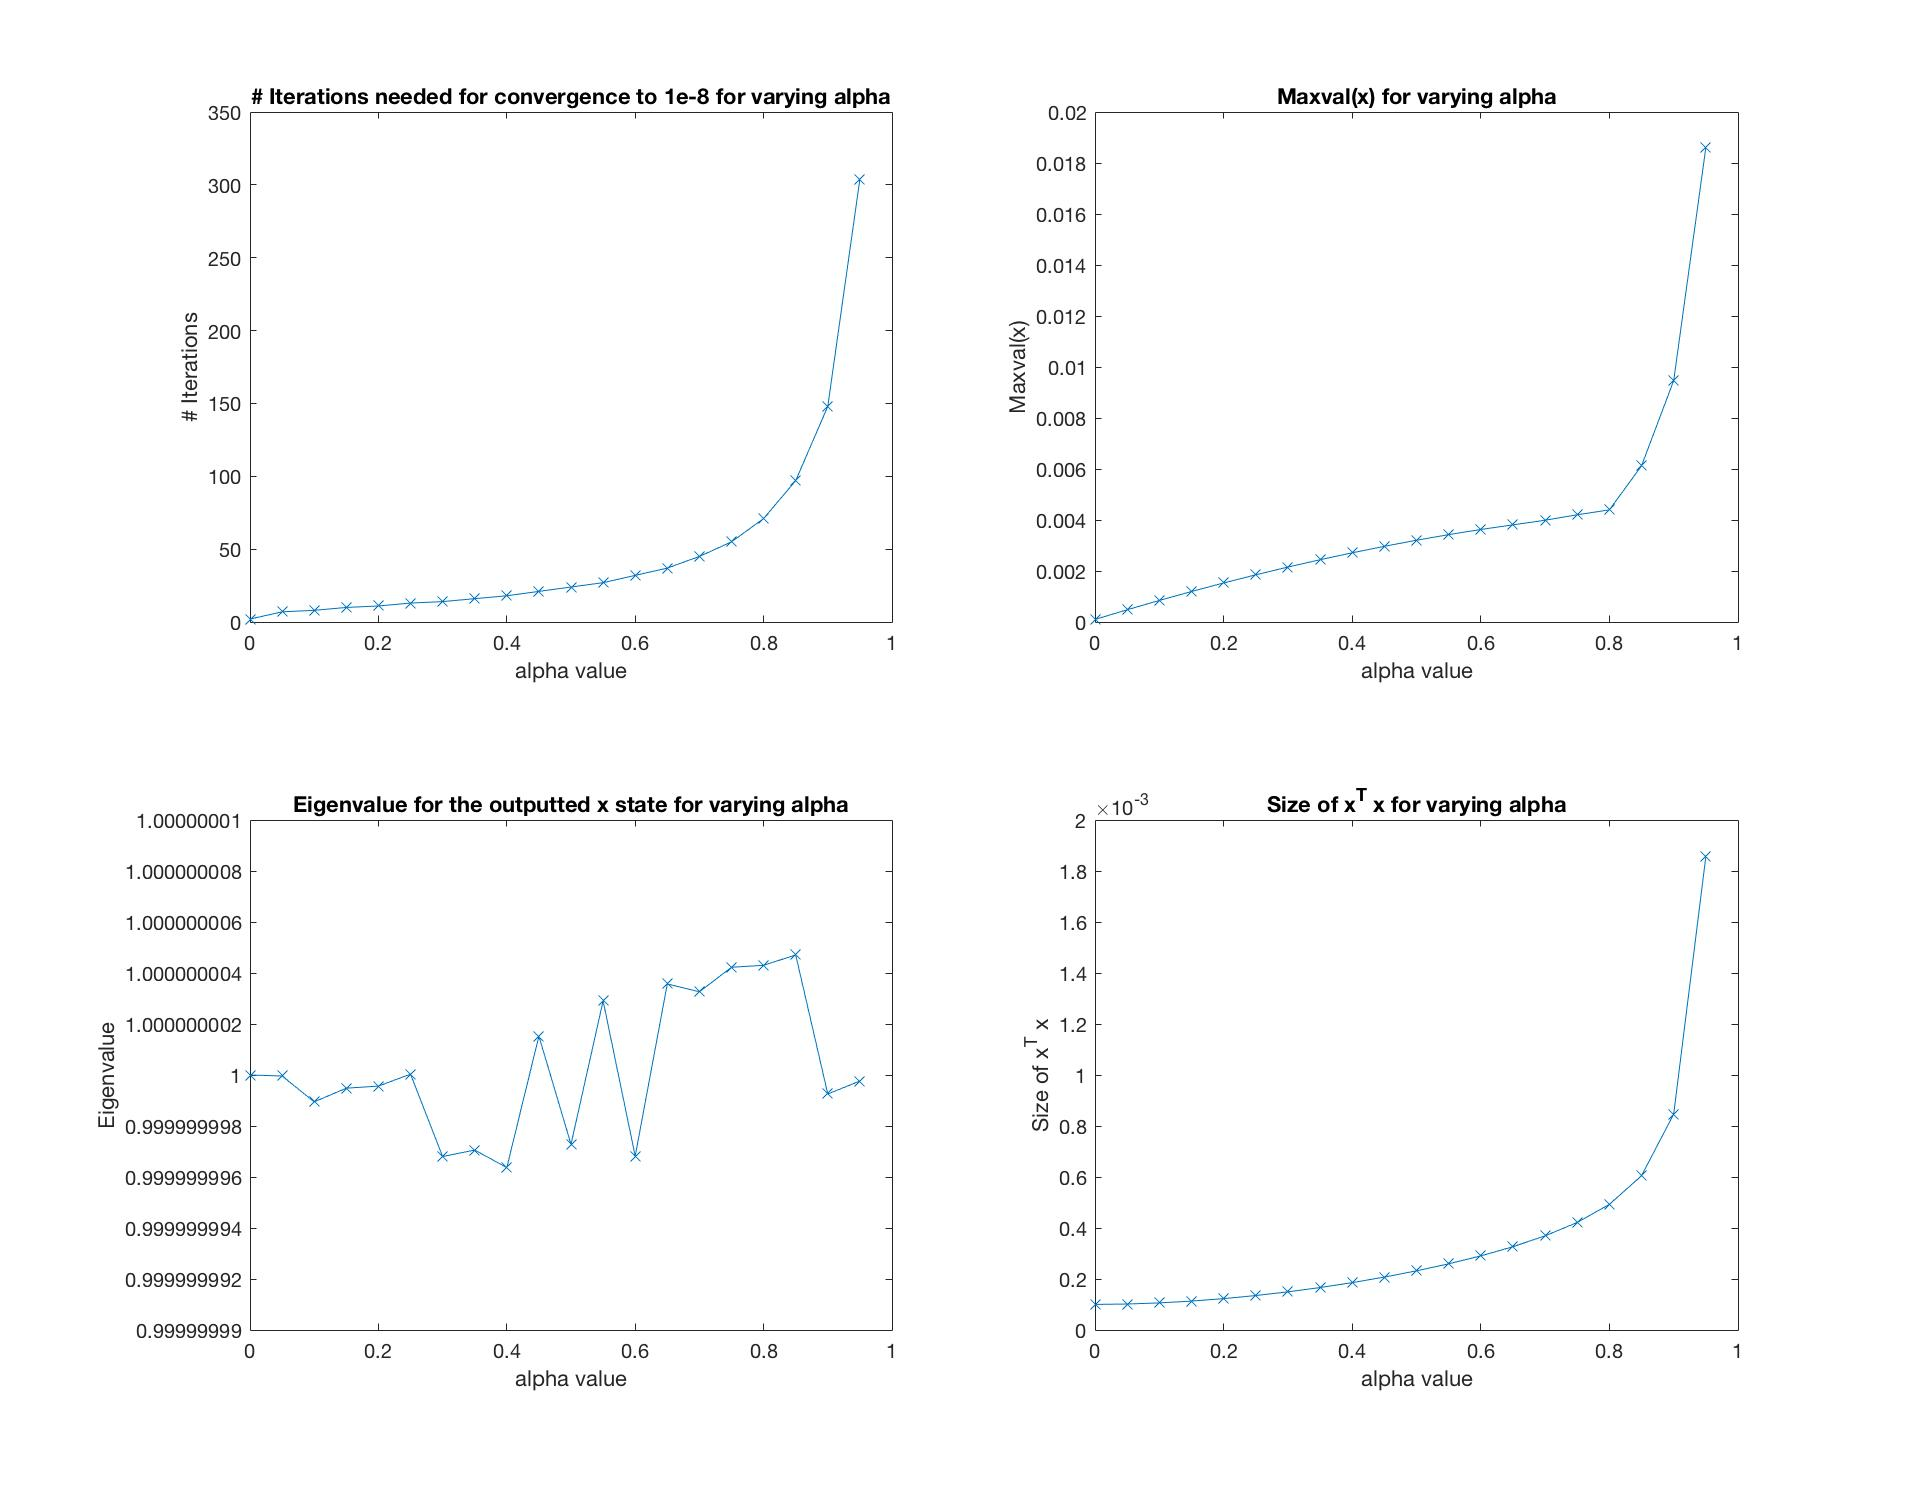
\includegraphics[width = \textwidth]{fig_varyingalpha}
				\caption{Various impacts of varying $\alpha$ in the PageRank algorithm} 
			\end{figure}
			Refer to figure 1.
		\begin{enumerate}
			\item It is clear that larger the value of $\alpha$ the more iterations it takes for the algorithm to converge. The number of iterations seems to shoot up just after the value of $\alpha = 0.85$.
			\item The maximum value of any page in the final state \textbf{x} increases with increasing $\alpha$ which suggests the algorithm gives a clearer view of the most dominant webpage for for larger values of $\alpha$. This is to be expected as larger values of $\alpha$ correspond to less randomized webpage surfing and more consistent behaviour of following the links on the current webpage.
			\item The values of $\lambda$ can be seen to near 1 for all $\alpha$ and thus are not significant.
			\item The value of $\textbf{x}^\star \textbf{x}$ can be seen to be increasing as $\alpha$ increases which again suggests PageRank converges to a more distinct vector for larger values of $\alpha$ and thus a more desirable result for ranking webpages.
			\end{enumerate}
			It seems that Page and Brin choose a value of $\alpha = 0.85$ because it is a compromise between having a more dominant eigenvector solution state, $\textbf{x}$, which is desirable and occurs for large values of $\alpha$, and reducing the number of operation counts needed for the answer to converge to a reasonable tolerance level, which increases quite dramatically for values of $\alpha > 0.85$.
			
			We know that power iteration converges at a rate of 
			$$
				|\frac{\lambda_2}{\lambda_1}|
			$$
			Since convergence takes longer for larger values of $\alpha$ and we know that $\lambda_1 = 1$, it must mean that $\lambda_2$ is increasing and getting closer - at an order greater than linearly - to the most dominant eigenvalue of $\lambda_1 = 1$.
			
			The files \texttt{q1c.m} and \texttt{PageRank.m} are used in this section.
		%%%%%%%%%%%%%%%%%%%%%%%%%%%%%%%%%%%%%%%%%%%%%%%%%%%%%%%%%%%%
		\item In the PageRank algorithm, at every step of the iteration $\textbf{x}^{(k)}$ is multiplied by $\textbf{P}^T$ to get $\textbf{x}^{(k+1)}$. The matrix-vector multiplication can be expanded and written as 
			\begin{equation*}
			\begin{split}
				\textbf{P}^T \textbf{x}^{(k)} 
				& = (\alpha \textbf{G} + \alpha \textbf{a1}^T/N + (1-\alpha) \textbf{11}^T /N )^T \textbf{x}^{(k)} \\
				& = (\alpha \textbf{G}^T + \alpha \textbf{1a}^T/N + (1-\alpha) \textbf{11}^T /N ) \textbf{x}^{(k)} \\
				& = \alpha \textbf{G}^T \textbf{x}^{(k)} + \alpha \textbf{1a}^T\textbf{x}^{(k)}/N + (1-\alpha) \textbf{11}^T \textbf{x}^{(k)} /N
			\end{split}
			\end{equation*}
			 Now it is possible to take advantage of the fact that $\textbf{G}$ is a sparse matrix in the calculation of 
			$$
				\alpha \textbf{G}^T \textbf{x}^{(k)}
			$$
			Furthermore since the rest of the matrix $\textbf{P}^T$ is composed of outer-products, the calculation is further sped up as
			$$
				\alpha \textbf{1a}^T\textbf{x}^{(k)}/N + (1-\alpha) \textbf{11}^T \textbf{x}^{(k)} /N 
				= (\alpha \textbf{1}(\textbf{a}^T\textbf{x}^{(k)}) + (1-\alpha) \textbf{1}(\textbf{1}^T \textbf{x}^{(k)}) )/N
			$$
			which reduces the multiplication to inner-products. \\
			Below is a graph of comparison in run-times for different values of $\alpha$. It is clear than the sparse PageRank method is faster, especially for larger values of $\alpha$.
			
			\begin{figure}[h!]
			\centering
				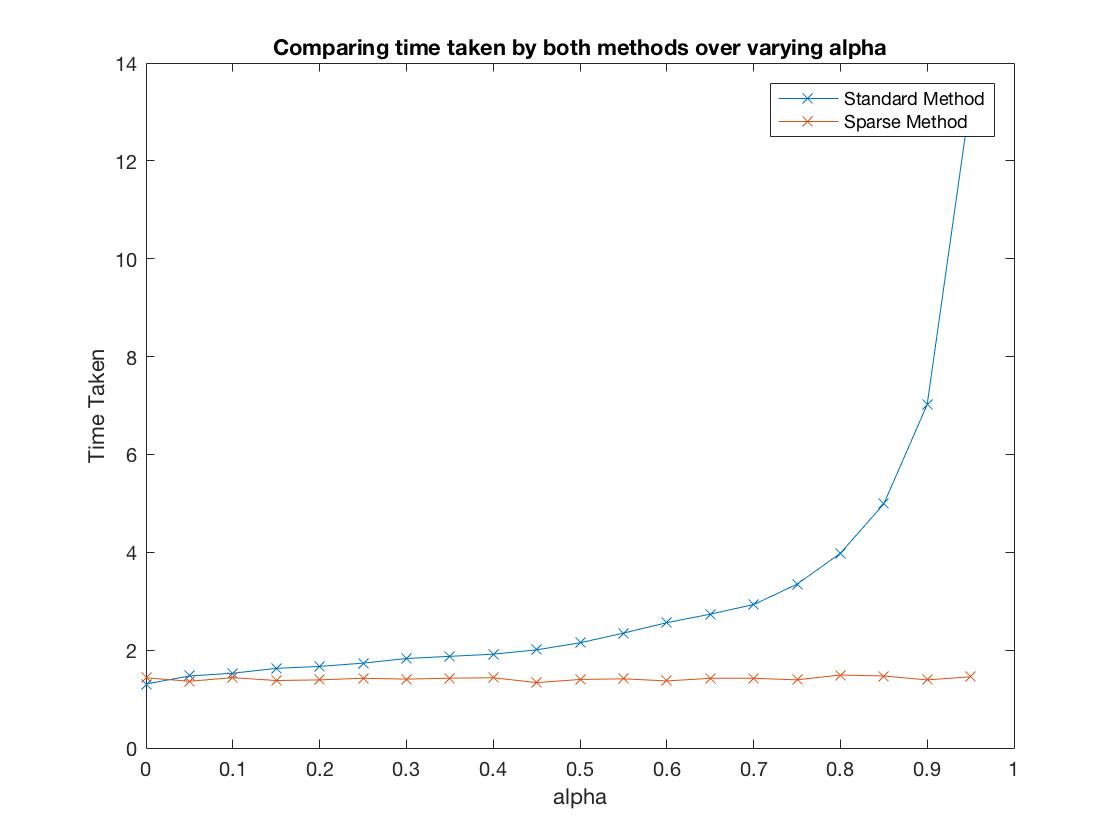
\includegraphics[width = 0.75\textwidth]{fig_timetaken}
				\caption{Time Taken comparison between the PageRank algorithm and a sparse PageRank algorithm}
			\end{figure}
			
			The files \texttt{PageRank.m}, \texttt{sparsePageRank.m}, \texttt{q1d.m}, and \texttt{q1d\_comparison.m} were used in this section.
	\end{enumerate}
	%%%%%%%%%%%%%%%%%%%%%%%%%%%%%%%%%%%%%%%%%%%%%%%%%%%%%%%%%%%%
	%%%%%%%%%%%%%%%%%%%%%%%%%%%%%%%%%%%%%%%%%%%%%%%%%%%%%%%%%%%%
	\item \textbf{Principal Component Analysis - Eigenworm} \\
		\begin{enumerate}
			\item The general householder algorithm computes each row and column separately and iterates over the entire inputted matrix. 
			
			The algorithm implemented in \texttt{modified\_house.m} takes into account the fact that the inputted matrix is symmetric and that it is known that outputted solution will be symmetric tridiagonal as well.
			
			Symmetry gives that each row and column of the solution vector will be the same and thus after a row is computed no operations are needed to compute the column and the values can simply be copied there.
			
			Sparsity gives that after the $k^\text{th}$ iteration only rows (and columns) $k:m$ need to be considered and not all rows (and columns) $1:m$. 
			
			Further implementation gains can be made by computing and storing values smartly.
			
			\textbf{T} will be a symmetric tridiagonal matrix and thus the table below provides the leading and first diagonal below - and also above due to symmetry - terms.
			 
\begin{table}[h]              
\centering                 
\begin{tabular}{|c|c|c|}
\hline
Position & Leading Diagonal & First Diagonal Below (and Above) \\     
\hline                     
1 & 9.8777e+03 & -2.3421e+04 \\
\hline                     
2 & 7.8779e+04 & -2.1425e+04 \\
\hline                     
3 & 3.0634e+04 & 1.0275e+04 \\ 
\hline                     
4 & 3.6216e+04 & -2.4093e+04 \\
\hline                     
5 & 3.6938e+04 & -1.8073e+04 \\
\hline                     
6 & 3.4697e+04 & -4.8259e+03 \\
\hline                     
7 & 2.9887e+03 & 1.0522e+03 \\ 
\hline                     
8 & 1.6612e+03 & 7.9013e+02 \\ 
\hline                     
9 & 1.4208e+03 & -5.7376e+02 \\
\hline                     
10 & 1.2237e+03 & -6.7347e+02 \\
\hline                     
11 & 1.4637e+03 & 5.6362e+02 \\ 
\hline                     
12 & 6.9743e+02 & 2.3686e+02 \\ 
\hline                     
13 & 4.0024e+02 & 1.8742e+02 \\ 
\hline                     
14 & 3.1895e+02 & -1.2315e+02 \\
\hline                     
15 & 2.2242e+02 & 1.2697e+02 \\ 
\hline                     
16 & 2.4602e+02 & -1.1024e+02 \\
\hline                     
17 & 1.8964e+02 & -8.6260e+01 \\
\hline                     
18 & 1.5931e+02 & 7.0396e+01 \\ 
\hline                     
19 & 1.2804e+02 & 6.7680e+01 \\ 
\hline                     
20 & 1.5134e+02 & 7.6119e+01 \\ 
\hline                     
21 & 1.4409e+02 & -5.7494e+01 \\
\hline                     
22 & 1.0892e+02 & -5.0201e+01 \\
\hline                     
23 & 1.0446e+02 & -4.6905e+01 \\
\hline                     
24 & 9.0199e+01 & 4.4424e+01 \\ 
\hline           
25 & 9.5351e+01 & -4.9741e+01 \\
\hline                     
26 & 1.1296e+02 & 5.5187e+01 \\ 
\hline                     
27 & 1.0323e+02 & 4.2793e+01 \\ 
\hline                     
28 & 8.0602e+01 & 3.5353e+01 \\     
\hline           
29 & 6.9611e+01 & 3.1304e+01 \\ 
\hline                     
\end{tabular}              
\caption{Values of T (continued in the next table)}   
\label{table:MyTableLabel} 
\end{table}   			

\begin{table}[h]              
\centering                 
\begin{tabular}{|c|c|c|}
\hline
Position & Leading Diagonal & First Diagonal Below (and Above) \\     
\hline                     
30 & 6.9129e+01 & 3.3566e+01 \\ 
\hline          
31 & 6.1415e+01 & -2.6871e+01 \\
\hline                     
32 & 5.6463e+01 & -2.8626e+01 \\
\hline                     
33 & 6.3152e+01 & -3.1846e+01 \\
\hline                     
34 & 6.1053e+01 & -2.3798e+01 \\
\hline                     
35 & 5.0833e+01 & -2.4951e+01 \\
\hline                     
36 & 4.6056e+01 & -2.1178e+01 \\
\hline                     
37 & 5.0741e+01 & -2.8561e+01 \\
\hline                     
38 & 5.8714e+01 & -2.4612e+01 \\
\hline                     
39 & 5.5031e+01 & 3.1549e+01 \\ 
\hline                     
40 & 6.4281e+01 & 2.9187e+01 \\ 
\hline                     
41 & 6.2629e+01 & -2.5914e+01 \\
\hline                     
42 & 4.5035e+01 & 2.2407e+01 \\ 
\hline                     
43 & 4.8882e+01 & -2.3896e+01 \\
\hline                     
44 & 5.1059e+01 & -2.6367e+01 \\
\hline                     
45 & 4.9927e+01 & -2.2886e+01 \\
\hline                     
46 & 4.4668e+01 & 2.1010e+01 \\ 
\hline                     
47 & 4.2934e+01 & 1.9811e+01 \\ 
\hline                     
48 & 5.0568e+01 & -3.0852e+01 \\
\hline                     
49 & 4.3834e+01 & \\ 
\hline                     
\end{tabular}              
\caption{Values of T}   
\label{table:MyTableLabel2} 
\end{table}   
	%%%%%%%%%%%%%%%%%%%%%%%%%%%%%%%%%%%%%%%%%%%%%%%%%%%%%%%%%%%%
	
			\item The QR algorithm can be used to find the eigenvalues of \textbf{T}. Using a shift method increases the rate of convergence. This gives two steps to the algorithm 
			 \begin{enumerate}
			 	\item Choosing which shift method to use. 
			 	 
			 	In lectures Rayleigh and Wilkinson shift are mentioned. Both have been implemented in the code and I found no significant difference (see code \texttt{q2a.m} for more information) and thus chose the Wilkinson shift.
			 	\item Choosing what QR algorithm to use to solve the linear system given by
			 	$$
			 		(A - \mu I)x = 0
			 	$$ 
			 	in each step of the QR algorithm. 
			 	
			 	One option is the modified gram schmidt algorithm which can be altered to take advantage of the sparse structure of \textbf{T}. But this gives the matrices Q and R which must then be multiplied and thus involves many FLOPs. 
			 	
			 	The second option is to use givens rotations to directly compute RQ. I used the information from \\ \texttt{http://zoro.ee.ncku.edu.tw/na/res/10-QR\_factorization.pdf} which taught me the method and helped outlined the relevant algorithm. This reduces the number of required FLOPs significantly. 
			 	
			 	I have chosen to use the modified modified gram schmidt algorithm for the Rayleigh shift method (if used) and the optimal givens rotation method for the Wilkinson shift method. 
			 \end{enumerate}
			
			I get the following 10 most dominant eigenvalues
			\begin{verbatim}
Most dominant eigenvalues (top 10)

1    9.3021e+04
2    6.7102e+04
3    3.8155e+04
4    2.3804e+04
5    6.1647e+03
6    2.8319e+03
7    2.2346e+03
8    1.6078e+03
9    9.5538e+02
10   6.3683e+02
			\end{verbatim}
		The magnitude of the 4 most dominant eigenvalues is an order of magnitude bigger than the next 4 most dominant eigenvalues. Furthermore the second 4 most dominant eigenvalues are an order of magnitude larger than the next dominant eigenvalues. This means that the data could be explained by the Principal components corresponding to these large eigenvalues. 
		
		This section uses \texttt{q2a.m}, \texttt{QR\_wilkinson.m}, \texttt{RQ\_givens.m}, and optionally \texttt{QR\_rayleighshift.m}and \texttt{mgs\_t.m}. Although to run \texttt{q2a.m} requires all the files in the folder \texttt{Eigenworm}.
			%%%%%%%%%%%%%%%%%%%%%%%%%%%%%%%%%%%%%%%%%%%%%%%%%%%%%%%%%%%%
		\item To find the eigenvectors associated with the eigenvalues found in the last part for \textbf{C}, $\textbf{C} - \lambda \textbf{I}$ can be decomposed using an LU decomposition. Since the equation of interest is $ (\textbf{C} - \lambda \textbf{I}) x = 0 $ once the LU decomposition has been found L can be discarded and only $U x = 0 $ is left. Since $C - \lambda I$ is singular it can be shown that $U(N,N) = 0$. To rectify this and perform backwards substitution this must be given a value $\neq 0$.
		
		\begin{figure}[h!]
		\centering
		\caption{eigenvectors corresponding to the 4 most dominant eigenvalues}	
		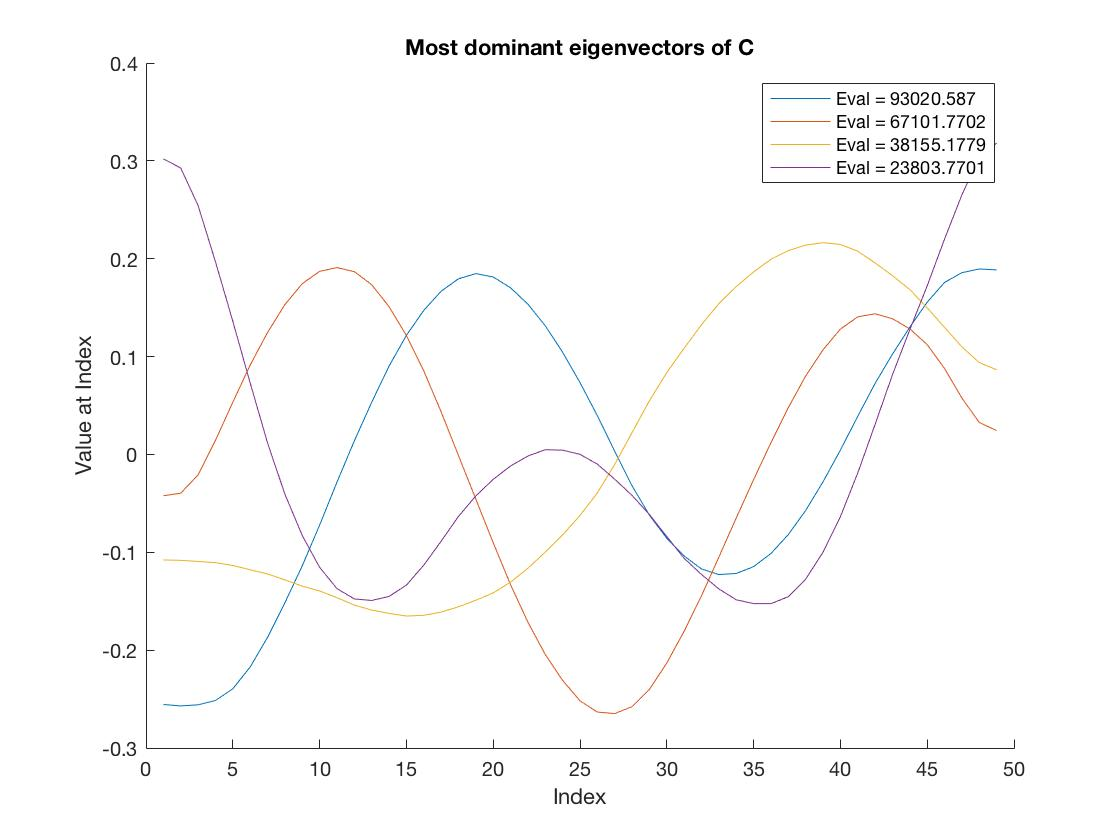
\includegraphics[width = 0.65\textwidth]{fig_evecs}
		\end{figure}

		A table of the values of the eigenvectors corresponding to the 4 most dominant eigenvalues is in the appendix.
		
			\item The projection coefficients are found using the method given in the paper. See \texttt{q2a.m} for more info. They are 
			\begin{verbatim}
Proj_Table = 

    Principal_Component    Coefficient
    ___________________    ___________

    1.0000e+00             -1.1813e+00
    2.0000e+00              2.4926e+00
    3.0000e+00             -8.4968e-01
    4.0000e+00              1.8638e+00
    5.0000e+00             -1.3084e+00
    6.0000e+00             -5.0532e-02
    7.0000e+00              2.0338e-02
    8.0000e+00              1.6361e-01
    9.0000e+00              2.7700e-01
    1.0000e+01             -1.0823e-01
   
			\end{verbatim}
			
			The first 5 projection coefficients are significantly larger than the next 5.
			
			The plot of the chosen principal components is
			
			\begin{figure}[h!]
				\centering
				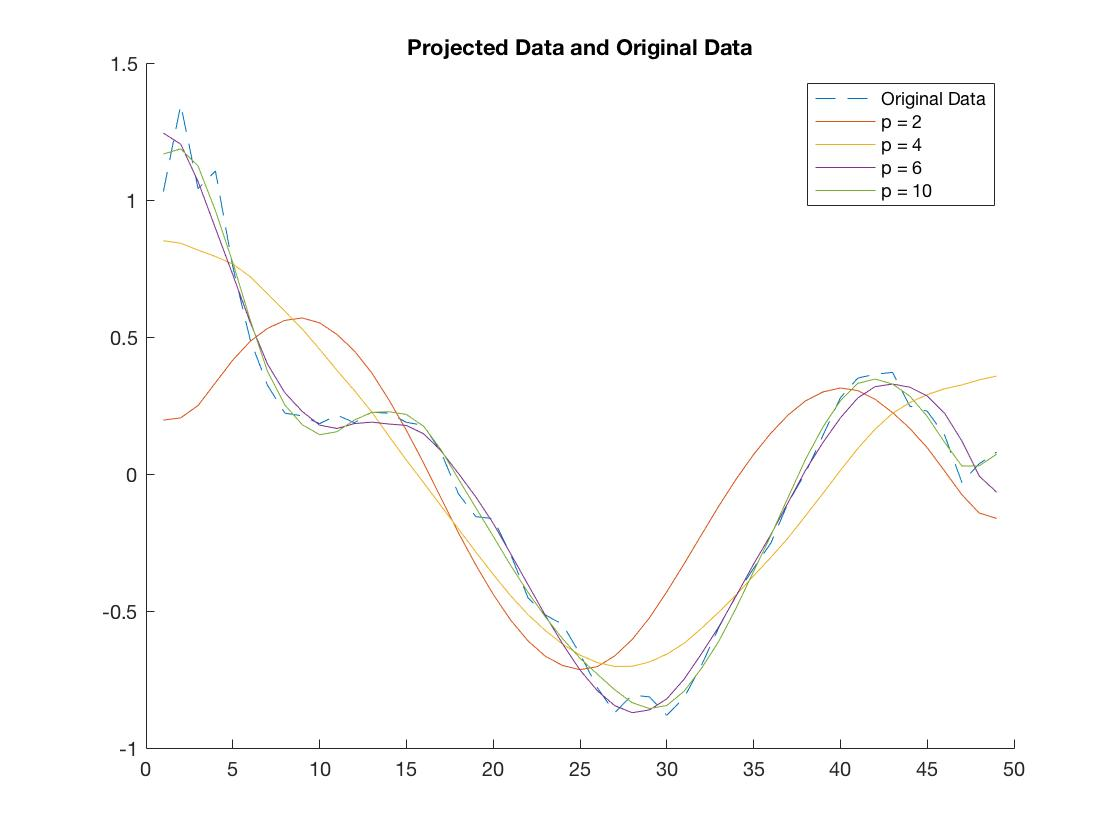
\includegraphics[width = 0.65\textwidth]{fig_data}
				\caption{Projected Data and Original Data}
			\end{figure}
			
			Choosing p is a balance between describing all aspects of the data and not trying to overfit the data. Also having a small value of p means that the data can be described relatively simply and thus concise explanations can be formed. This can be hard if there are a large number of Principal Components. 
			
			The error table for each principal component is
			
			\begin{verbatim}
Error_Table = 

    Principal_Component      Error   
    ___________________    __________

    1.0000e+00             1.2373e+01
    2.0000e+00             6.1598e+00
    3.0000e+00             5.4379e+00
    4.0000e+00             1.9640e+00
    5.0000e+00             2.5213e-01
    6.0000e+00             2.4957e-01
    7.0000e+00             2.4916e-01
    8.0000e+00             2.2239e-01
    9.0000e+00             1.4566e-01
    1.0000e+01             1.3395e-01
			\end{verbatim}
			
			The error table shows that until p = 6 the error falls quite steadily and gradually this rate decreases. This suggests that a value of p = 6 would be a good choice. Also it can be seen from the graph that the 6th eigenvector fits the original data quite well. Once might argue that 10th eigenvector fits the data quite well as well but perhaps will lead to overfitting as can be seen by its less smooth shape. On balance I believe a good choice would be p = 6.
			  		
			\texttt{q2a.m} and \texttt{evec.m} are used in this part			
		\end{enumerate}
	%%%%%%%%%%%%%%%%%%%%%%%%%%%%%%%%%%%%%%%%%%%%%%%%%%%%%%%%%%%%

	\item \textbf{Mastery}
	\begin{enumerate}
		\item First note that $ (\textbf{P}^T \textbf{D}_2 \textbf{P}) = A $ is a banded matrix. It can further be shown that A is a positive semi-definite matrix. Thus a banded gaussian elimination LU decomposition approach is chosen. This is because the band width (upper and lower) of A is 2 and thus the decomposition will only take $2pqN$ points where $p = 2$ and $q = 2$. Thus in total this will require $8N$ FLOPs. 
		 
			After the decomposition, forwards and backwards substitution can be simplified to to make sure of the sparsity of L and U. L and U are sparse because A is symmetric and thus L and U only have terms on the two diagonals above or below the leading diagonal. 
			
			Forward substitution requires $ 2 + 3(N-2)$ FLOPs. 
			
			Backwards substitution requires $3 + 4(N-2)$ FLOPs. 
			
			All this together gives an algorithm that solves the system in $15N - 9 $ FLOPs. This is a linear scaling algorithm, $O(N)$.
			
		\item The algorithm used is in \texttt{algo\_mastery.m}. We can use algorithm even though $D_2$ is singular because of the zero mean condition (ZMC). Also the algorithm gives that after doing an LU decomposition $U(N,N) = 0$ but we change to be 1 due to ZMC much like in the previous project. 
		
		A table of the errors and scaled error (by size of the problem) is produced using this algorithm below
		
		\begin{verbatim}
Error_Table = 

        N           Error   
    __________    __________

    1.6000e+01    2.2955e-02
    3.2000e+01    5.7055e-03
    6.4000e+01    1.4243e-03
    1.2800e+02    3.5595e-04


ScaledError_Table = 

        N         Scaled_Error
    __________    ____________

    1.6000e+01    5.8764e+00  
    3.2000e+01    5.8424e+00  
    6.4000e+01    5.8340e+00  
    1.2800e+02    5.8318e+00  
		\end{verbatim}
		
		\item 
		algoMastery: algorithm implemented in this part of the current project
		
		algoFft: algorithm implemented in previous project using fast fourier transforms
		
		algoP4: algorithm implemented in part 4 of the previous project using the eigenvalues and eigenvectors approach
		
		algoP1: algorithm implemented in part 1 of the previous project using the initial approach.
		 		
		algoMastery is $O(N)$ which is much better than algoP4 that was $O(N^2)$. algoFft was $ N log(N)$ and thus actually faster than algoMastery for most values of N except when N gets absurdly large. $log(2^{15}) \approx 10 < 15N$ for $N<2^{15}$. 
		
		\begin{figure}[h!]
			\centering
			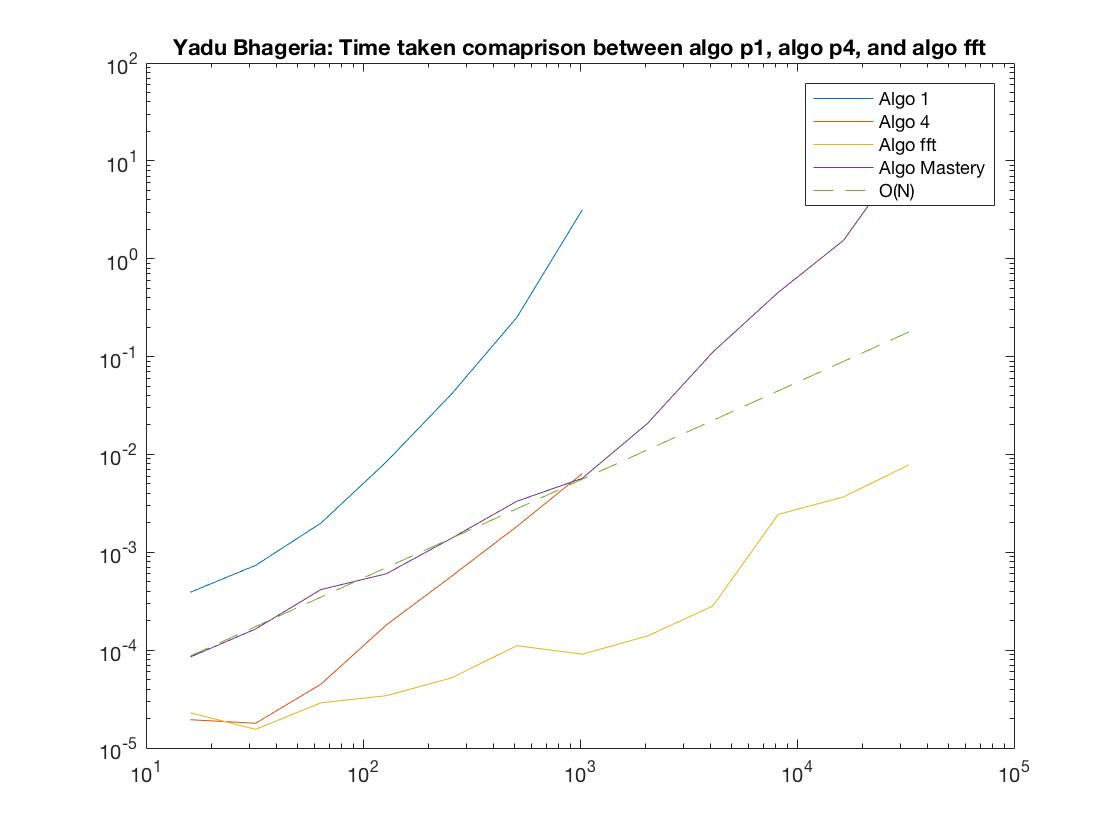
\includegraphics[width = 0.75\textwidth]{fig_1e15.jpg}
			\caption{Runtimes for the various algorithms implemented to solve this problem}
		\end{figure} 
		
		The figure indicates that algoP4 is faster than algoMastery for values upto $2^{10}$ after which it would seem that algoMastery would overtake algoP4. This is likely due to vector matrix multiplication being a very efficient operation with low memory movement whereas algoMastery would require significantly more memory movement. But nonetheless algoMastery scales better. 
		
		algoFft does surprisingly well. This is likely due to it being highly optimised and again not requiring much memory movement as the problem size increases. 
		
		One advantage of algoMastery implemented right now using the banded LU decomposition method for symmetric matrices is that it scales very well. i.e. $O(N)$ and thus should theoretically be the fastest algorithm of those implemented for a massive problem size. 
		
		Another is that since algoMastery is dealing with banded matrices it would be feasible to create an algorithm that doesn't use a NxN matrix to store data and instead uses multiple vectors. This would considerably speed up the algorithm and make use of the sparsity of the matrices. Unfortunately I have not been able to make use of this fact in the current project due to time restraints but it doesnt change the fact that it is a definitely advantage of the banded LU decomposition method. 
		
		One drawback of banded LU decomposition is that it is only really fast for small band sizes. If A were not of upper and lower band size equal to 2 then the algorithm would eventually degenerate to a normal LU decomposition algorithm (for large band sizes) and thus be of higher order.
		
		All the files in the mastery folder are needed for these parts of the project.
		
	\end{enumerate}
\end{enumerate}
\newpage
\section{Appendix}

\begin{table}[h!]                                              
\centering                                                  
\begin{tabular}{|c|c|c|c|c|}                                
\hline
Index & Eigenvector 1 & Eigenvector 2 & Eigenvector 3 & Eigenvector 4 \\
\hline                                                      
1 & -2.5558e-01 & -4.2214e-02 & -1.0782e-01 & 3.0207e-01 \\ 
\hline                                                      
2 & -2.5699e-01 & -3.9614e-02 & -1.0825e-01 & 2.9267e-01 \\ 
\hline                                                      
3 & -2.5586e-01 & -2.0955e-02 & -1.0936e-01 & 2.5435e-01 \\ 
\hline                                                      
4 & -2.5142e-01 & 1.4361e-02 & -1.1059e-01 & 1.9693e-01 \\  
\hline                                                      
5 & -2.3953e-01 & 5.3306e-02 & -1.1352e-01 & 1.3615e-01 \\  
\hline                                                      
6 & -2.1722e-01 & 9.1278e-02 & -1.1784e-01 & 7.3045e-02 \\  
\hline                                                      
7 & -1.8701e-01 & 1.2457e-01 & -1.2213e-01 & 1.1835e-02 \\  
\hline                                                      
8 & -1.5166e-01 & 1.5307e-01 & -1.2820e-01 & -4.0605e-02 \\ 
\hline                                                      
9 & -1.1384e-01 & 1.7449e-01 & -1.3456e-01 & -8.2824e-02 \\ 
\hline                                                      
10 & -7.2282e-02 & 1.8709e-01 & -1.3955e-01 & -1.1539e-01 \\
\hline                                                      
11 & -2.8330e-02 & 1.9090e-01 & -1.4639e-01 & -1.3712e-01 \\
\hline                                                      
12 & 1.3792e-02 & 1.8679e-01 & -1.5395e-01 & -1.4768e-01 \\ 
\hline                                                      
13 & 5.3266e-02 & 1.7346e-01 & -1.5909e-01 & -1.4924e-01 \\ 
\hline                                                      
14 & 9.0185e-02 & 1.5094e-01 & -1.6243e-01 & -1.4512e-01 \\ 
\hline                                                      
15 & 1.2164e-01 & 1.2155e-01 & -1.6515e-01 & -1.3356e-01 \\ 
\hline                                                      
16 & 1.4721e-01 & 8.5364e-02 & -1.6440e-01 & -1.1318e-01 \\ 
\hline                                                      
17 & 1.6676e-01 & 4.3515e-02 & -1.6109e-01 & -8.8697e-02 \\ 
\hline                                                      
18 & 1.7950e-01 & -1.1847e-03 & -1.5568e-01 & -6.3303e-02 \\
\hline                                                      
19 & 1.8478e-01 & -4.5754e-02 & -1.4900e-01 & -4.2383e-02 \\
\hline                                                      
20 & 1.8131e-01 & -9.0234e-02 & -1.4149e-01 & -2.5446e-02 \\
\hline                                                      
21 & 1.7027e-01 & -1.3312e-01 & -1.3050e-01 & -1.1837e-02 \\
\hline                                                      
22 & 1.5351e-01 & -1.7147e-01 & -1.1632e-01 & -1.5935e-03 \\
\hline                                                      
23 & 1.3144e-01 & -2.0452e-01 & -9.9747e-02 & 4.8368e-03 \\ 
\hline                                                      
24 & 1.0436e-01 & -2.3097e-01 & -8.2156e-02 & 4.3284e-03 \\ 
\hline                                                      
25 & 7.3372e-02 & -2.5175e-01 & -6.2368e-02 & 1.1276e-04 \\ 
\hline                                                      
26 & 3.9566e-02 & -2.6330e-01 & -3.9292e-02 & -9.9579e-03 \\
\hline                                                      
27 & 3.2131e-03 & -2.6481e-01 & -1.0213e-02 & -2.5341e-02 \\
\hline                                                      
28 & -3.2089e-02 & -2.5772e-01 & 2.2365e-02 & -4.1958e-02 \\
\hline                                                      
29 & -6.2169e-02 & -2.4007e-01 & 5.4886e-02 & -6.1486e-02 \\
\hline                                                      
30 & -8.5751e-02 & -2.1311e-01 & 8.3649e-02 & -8.3926e-02 \\
\hline                                           
\end{tabular}                                               
\caption{Eigenvectors corresponding to the 4 most dominant eigenvalues (continued in next table)}                                    
\label{table:MyTableLa22bel}                                  
\end{table} 

\begin{table}[h!]                                            
\centering                                                  
\begin{tabular}{|c|c|c|c|c|}                                
\hline
Index & Eigenvector 1 & Eigenvector 2 & Eigenvector 3 & Eigenvector 4 \\
\hline                                                      
31 & -1.0389e-01 & -1.8063e-01 & 1.0855e-01 & -1.0626e-01 \\
\hline                                                      
32 & -1.1702e-01 & -1.4435e-01 & 1.3264e-01 & -1.2269e-01 \\
\hline                                                      
33 & -1.2276e-01 & -1.0492e-01 & 1.5418e-01 & -1.3747e-01 \\
\hline                                                      
34 & -1.2161e-01 & -6.4961e-02 & 1.7156e-01 & -1.4853e-01 \\
\hline                                                      
35 & -1.1468e-01 & -2.5805e-02 & 1.8651e-01 & -1.5244e-01 \\
\hline                                                      
36 & -1.0122e-01 & 1.2005e-02 & 1.9948e-01 & -1.5248e-01 \\ 
\hline                                                      
37 & -8.1860e-02 & 4.7827e-02 & 2.0829e-01 & -1.4534e-01 \\ 
\hline                                                      
38 & -5.7268e-02 & 8.0163e-02 & 2.1392e-01 & -1.2743e-01 \\ 
\hline                                                      
39 & -2.7931e-02 & 1.0694e-01 & 2.1636e-01 & -9.9878e-02 \\ 
\hline                                                      
40 & 4.4074e-03 & 1.2806e-01 & 2.1460e-01 & -6.3598e-02 \\  
\hline                                                      
41 & 3.8946e-02 & 1.4064e-01 & 2.0766e-01 & -1.8897e-02 \\  
\hline                                                      
42 & 7.2605e-02 & 1.4374e-01 & 1.9564e-01 & 3.0712e-02 \\   
\hline                                                      
43 & 1.0252e-01 & 1.3865e-01 & 1.8271e-01 & 8.1527e-02 \\   
\hline                                                      
44 & 1.3008e-01 & 1.2827e-01 & 1.6837e-01 & 1.2755e-01 \\   
\hline                                                      
45 & 1.5561e-01 & 1.1221e-01 & 1.4980e-01 & 1.7226e-01 \\   
\hline                                                      
46 & 1.7581e-01 & 8.7740e-02 & 1.2977e-01 & 2.2011e-01 \\   
\hline                                                      
47 & 1.8575e-01 & 5.7553e-02 & 1.0980e-01 & 2.6532e-01 \\   
\hline                                                      
48 & 1.8950e-01 & 3.2627e-02 & 9.3869e-02 & 3.0370e-01 \\   
\hline                                                      
49 & 1.8858e-01 & 2.4349e-02 & 8.6472e-02 & 3.1816e-01 \\   
\hline                                                      
\end{tabular}                                               
\caption{Continued Eigenvectors corresponding to the 4 most dominant eigenvalues}                                    
\label{table:MyTableLa22bel}                                  
\end{table} 
	
\end{document}